
% Sezione con i comandi per CREARE le tabelle.
% Note per noi:
% - L'attributo "Spedizione" di Fattura è NULLable
% - Le tabelle Vendita e Acquisto non hanno rispettivamente Cliente e Fornitore perchè i loro riferimenti sono già negli attributi Destinatario e Emittente della relativa Fattura

\vspace{1cm} % spazio bianco
% NOTA: gli spazi sono sotto sono degli spazi, non TAB, altrimenti non si vedono sul pdf
\begin{verbatim}
create table utente(
  username varchar(20) primary key,
  nome varchar(20),
  cognome varchar(20),
  indirizzo varchar(50),
  password varchar(20),
  email varchar(20)
);
\end{verbatim}

\noindent\makebox[\textwidth]{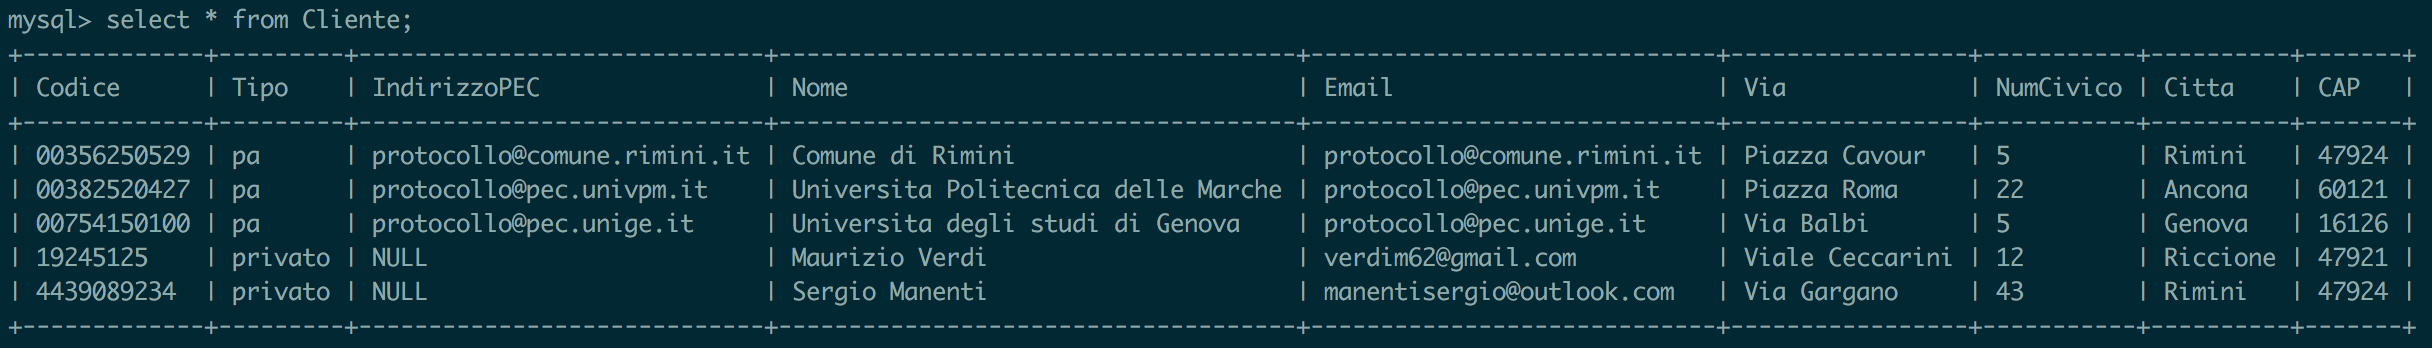
\includegraphics[page=1, width=0.7\linewidth]{./immagini/1}}
\newline\newline

\begin{verbatim}
create table utente(
  username varchar(20) primary key,
  nome varchar(20),
  cognome varchar(20),
  indirizzo varchar(50),
  password varchar(20),
  email varchar(20)
);
\end{verbatim}

\noindent\makebox[\textwidth]{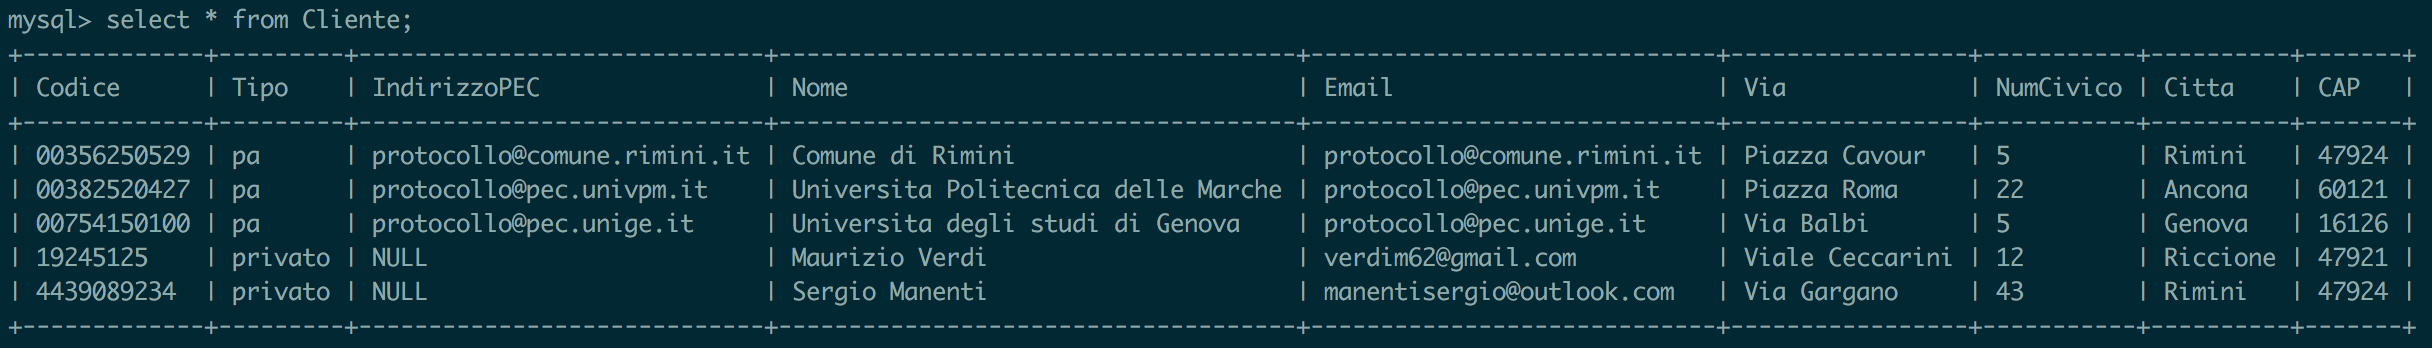
\includegraphics[page=1, width=0.7\linewidth]{./immagini/1}}
\newline\newline
